\documentclass[practic, labs]{BMSTU-IU7}

\usepackage{biblatex}
\usepackage{listings}
\usepackage{csvsimple}
\usepackage{caption}
\usepackage{pgfplots}
\pgfplotsset{compat=1.9}

\usepackage{geometry}
\geometry{verbose,a4paper,bmargin=2cm}

\newcommand{\code}[1]{\texttt{#1}}

\lstset{
	language=C++,
	numbers=left,
	captionpos=t,
	frame=single,  % Отображение рамки вокруг кода
	backgroundcolor=\color{white}
}

\student{Дьяченко А. А.}
\group{ИУ7-53Б}
\labsNumber{3}
\theme{<<Трудоёмкость сортировок>>}
\speciality{<<Анализ алгоритмов>>}
\supervisor{Строганов Д. В.}

\addbibresource{biblio.bib}


\begin{document}
	\maketitle

	\include{01-contents}
	\section*{ВВЕДЕНИЕ}
\addcontentsline{toc}{section}{ВВЕДЕНИЕ}

Сортировка --- это последовательное расположение или разбиение на группы чего-либо в зависимости от выбранного критерия \cite{вашинко2018блинная}.

Любой алгоритм сортировки можно разбить на три основные части:
\begin{itemize}
	\item сравнение элементов для определения их упорядоченности;
	\item перестановка элементов;
	\item сортирующий алгоритм, который осуществляет сравнение и перестановку элементов до тех пор, пока все элементы не будут упорядочены.
\end{itemize}
	
Цель лабораторной работы –-- изучить и исследовать трудоемкость алгоритмов сортировки.

Для достижения поставленных целей ставятся задачи:

\begin{itemize}
	\item реализация требуемых алгоритмов сортировки: блинная, выбором, перемешиванием;
	\item сравнение требуемого времени выполнения реализуемых алгоритмов в тактах процессора и занимаемой памяти;
	\item подготовка отчёта по лабораторной работе.
\end{itemize}
	\section{Аналитическая часть}

Расстояние Дамерау--Левенштейна представляет собой метрику, измеряющую разницу между двумя строками, путем подсчета минимального числа операций, необходимых для преобразования одной строки в другую.
Эти операции включают в себя вставку, удаление, замену символов и дополнительную относительно расстояния Левенштейна операцию, которая называется транспозицией, которая представляет собой перестановку двух соседних символов в строке. \cite{cyberleninka_modifitsirovannyi_algoritm}

Обозначения редакторских операций:
\begin{enumerate}
	\item I - вставка символа (insert);
	\item D - удаление (delete);
	\item R - замена (replace);
	\item M - совпадение двух символов (match);
	\item T - транспозиция двух соседних символов (transposition).
\end{enumerate}
I, D, R, T - штраф 1 (в преобразуемой строке).

Совпадение символа с самим собой не имеет дополнительной стоимости и оценивается как 0.

Эти операции и их стоимости позволяют вычислить расстояние Дамерау--Левенштейна между двумя строками, что является важным инструментом в областях, где требуется измерять сходство или различие между текстовыми последовательностями.

\subsection{Нерекурсивный алгоритм поиска расстояния Левенштейна}
Пусть $L1$ - длина строки $S_{1}$, $L2$ - длина строки $S_{2}$. 
$S_{1}[1..i]$ - подстрока $S_{1}$ с длиной $i$ символов, начиная с первого, $S_{2}[1..j]$ - подстрока $S_{2}$ длиной $j$ символов, начиная с первого. \cite{levenstein_book}

Расстояние Левенштейна может быть найдено с помощью формулы:

\begin{equation}
	\label{eq:d}
	D(i, j) = \begin{cases} 
		\max(i, j) &\text{если }\min(i, j) = 0, \\
		\min \lbrace \\
	     \qquad D(i, j-1) + 1, \\
	     \qquad D(i-1, j) + 1, \\
	     \qquad D(i-1, j-1) + m(S_{1}[i], S_{2}[j]), &\text{иначе} \\
	     \rbrace
	\end{cases},
\end{equation}

где $m(S_{1}[i], S_{2}[i])$ равна нулю, если $S_{1}[i] = S_{2}[i]$ и единице в противном случае.

Для оптимизации вычисления расстояния между строками используется матрица промежуточных значений. Её размерность определяется как $(len(S_{1}) + 1) × (len(S_{2}) + 1)$.
Каждая ячейка матрицы, обозначенная как $matrix[j, j]$, содержит значение расстояния между подстроками $S_{1}[1...i] и S_{2}[1...j]$. 
Первая строка и первый столбец этой матрицы представляют собой тривиальные случаи и соответствуют наибольшим f $i$ или $j$ в соответствующей строке или столбце.

Матрица заполняется в соответствии со следующей формулой:

\begin{equation}
	\label{eq:mat}
	M[i][j] = min \begin{cases}
		\qquad M[i-1][j] + 1,\\
		\qquad M[i][j-1] + 1,\\
		\qquad M[i-1][j-1] + m(S_{1}[i], S_{2}[j])\\
	\end{cases}.
\end{equation}

Расстоянием Левенштейна будет значение в самой правой нижней ячейке матрицы с индексами $i = len(S_{1}), j = len(S_{2})$.

\subsection{Нерекурсивный алгоритм поиска расстояния Дамерау--Левенштейна}

Расстояние Дамерау--Левенштейна между двумя строками, обозначенными как $S_1$ и $S_2$, может быть вычислено с использованием формулы \ref{eq:d1}. 
Эта формула имеет следующий вид:

\begin{equation}
    \begin{aligned}
        \label{eq:d1}
        \llap{$D(i, j) =$} 
        \begin{cases}
            \min(i, j) = 0, &\text{если} \max(i, j),\\
            \min \left\{ 
                \begin{array}{l}
                    D(i, j-1) + 1,\\
                    D(i-1, j) + 1,\\
                    D(i-1, j-1) + m(S_{1}[i], S_{2}[j]), 
                \end{array}
            \right. & \text{иначе}\\
            \left[ 
                \begin{array}{ll}
                    D(i-2, j-2) + 1, &\text{если }i,j > 1;\\
                    &S_{1}[i] = S_{2}[j-1];\\
                    &S_{1}[i-1] = S_{2}[j]\\
                    \infty, & \text{иначе}
                \end{array}
            \right.
        \end{cases},
    \end{aligned}
\end{equation}


Эта формула представляет собой рекуррентное соотношение, которое позволяет вычислить расстояние между двумя строками, учитывая вставки, удаления, замены и транспозиции символов. 
В результате выполнения этой формулы получается матрица, где значение в ячейке с индексами $i = len	(S_{1})$ и $j = len(S_{2})$ представляет собой расстояние Дамерау--Левенштейна между исходными строками $S_{1}$ и $S_{2}$.

Формула \ref{eq:d1} выводится на основе аналогичных рассмотрений, что и формула \ref{eq:d}, но с учетом дополнительной редакторской операции - транспозиции символов. 
Эта формула позволяет эффективно находить расстояние Дамерау--Левенштейна и широко используется в задачах редактирования и сравнения строк.

\newpage
\subsection{Рекурсивный алгоритм нахождения расстояния Дамерау--Левенштейна}

Рекурсивный алгоритм для вычисления расстояния Дамерау--Левенштейна реализует формулу \ref{eq:d1}. Функция $D$ определяется следующим образом:

\begin{enumerate}[label=\arabic*)]
	\item перевод из пустой строки в пустую строку не требует никаких операций и, следовательно, имеет стоимость равную нулю;
	\item перевод из пустой строки в строку $S_{1}$ требует выполнения $|S_{1}|$ операций, каждая из которых добавляет один символ к строке $S_{1}$. Таким образом, общая стоимость такого перевода равна $|S_{1}|$;
	\item перевод из строки $S_{1}$ в пустую строку аналогично требует выполнения $|S_{1}|$ операций удаления, каждая из которых удаляет один символ из строки $S_{1}$. Следовательно, общая стоимость такого перевода также равна $|S_{1}|$;
	\item для перевода из строки $S_{1}$ в строку $S_{2}$ требуется выполнить последовательность операций (удаление, вставка, замена, транспозиция) в определенной последовательности.
\end{enumerate}

Полагая $S_{1}'$ и $S_{2}'$ как строки $S_{1}$ и $S_{2}$ без их последних символов соответственно, цена преобразования из строки $S_{1}$ в строку $S_{2}$ может быть выражена следующими случаями:
\begin{enumerate}
   \item сумма цены преобразования строки $S_{1}'$ в $S_{2}$ и цены операции удаления, необходимой для преобразования $S_{1}'$ в $S_{1}$;
   \item сумма цены преобразования строки $S_{1}$ в $S_{2}'$ и цены операции вставки, необходимой для преобразования $S_{2}'$ в $S_{2}$;
   \item сумма цены преобразования из $S_{1}'$ в $S_{2}'$ и цены операции замены, предполагая, что последние символы $S_{1}$ и $S_{2}$ разные;
   \item цена преобразования из $S_{1}'$ в $S_{2}'$, предполагая, что последние символы $S_{1}$ и $S_{2}$ совпадают;
   \item сумма цены преобразования $S_{1}''$ в $S_{2}''$, предполагая, что последние два символа $S_{1}$ можно преобразовать путем транспозиции в два последних символа $S_{2}$.
\end{enumerate}

Таким образом, рекурсивный алгоритм находит оптимальное решение, учитывая все возможные варианты операций.

\subsection{Рекурсивный алгоритм с кэшированием для нахождения расстояния Дамерау--Левенштейна}

Рекурсивный алгоритм с кэшированием является улучшенной версией рекурсивного алгоритма нахождения расстояния Дамерау--Левенштейна. 
Он использует ту же формулу \ref{eq:d1}, но с добавлением механизма кэширования, чтобы избежать повторных вычислений и снизить вычислительную сложность.

Функция $D$ в этой версии алгоритма хранит результаты вычислений в специальной матрице кэша. 
Каждый элемент этой матрицы соответствует значениям $D(i, j)$ для определенной пары индексов $i$ и $j$. 
Если значение уже было вычислено, оно сохраняется в кэше, и при необходимости оно просто извлекается из кэша, вместо того чтобы пересчитываться заново.

Такой подход существенно ускоряет процесс вычисления расстояния Дамерау--Левенштейна, особенно при работе с большими строками.
Эффективное использование кэширования позволяет избежать множественных повторных вычислений и сделать алгоритм более производительным.

Таким образом, рекурсивный алгоритм с кэшированием представляет собой оптимизированную версию рекурсивного алгоритма, способную эффективно находить расстояние Дамерау--Левенштейна между двумя строками.

	\section{Конструкторская часть}

В этом разделе будут представлены схемы и/или псевдокоды реализуемых алгоритмов.

\subsection{Требования к ПО}
К программе предъявляется ряд требований:
\begin{itemize}[]
	\item искомая подстрока имеет размер $S$ от 6 до 10 символов;
	\item первые две пары символов искомой подстроки совпадают;
	\item при генерации исходной строки шанс 7/8 сгенерировать подстроку из $S$ случайных символов;
	\item при генерации исходной строки шанс 1/8 сгенерировать искомую подстроку, конкотенирующую с её первой парой символов, т.е. получить подстроку длины $S + 2$ символов;
	\item на вход подается строка и искомая в ней подстрока;
	\item на выходе требуется получить файл с записями индексов вхождения подстроки.
	
\end{itemize}

\newpage
\subsection{Разработка алгоритмов}

В листинге~\ref{alg:standart} рассмотрен псевдокод стандартного алгоритма поиска подстроки в строке.

\begin{algorithm}[H]
	\caption{Стандартный алгоритм}
	\label{alg:standart}
	\SetAlgoLined
	\KwIn{Строка $text$, подстрока $pattern$}
	\KwOut{Индекс первого вхождения $pattern$ в $text$, или -1 если не найден}
	$n \gets \text{length}(text)$\;
	$m \gets \text{length}(pattern)$\;
	\For{$i \gets 1$ \KwTo $n - m + 1$}{
		$j \gets 1$\;
		\While{$j \leq m$ \textbf{and} $text[i + j - 1] = pattern[j]$}{
			$j \gets j + 1$\;
		}
		\If{$j > m$}{
			\KwRet{$i$}\;
		}
	}
	\KwRet{-1}\;
\end{algorithm}

\newpage

Алгоритм Кнута-Морриса-Пратта поиска подстроки в строке использует префиксную функцию. 
Префиксная функция, вычисляемая для искомой подстроки, содержит сведения о том, в какой мере образец совпадает сам с собой после сдвигов. 
Эта информация помогает избежать лишних проверок при поиске~\cite{алексеенко2010информационная}.

В листинге~\ref{alg:pre} рассмотрен псевдокод алгоритма расчета префиксного массива.

\begin{algorithm}[H]
	\caption{Расчет префиксного массива}
	\label{alg:pre}
	\SetAlgoLined
	\KwIn{Подстрока $x$}
	\KwOut{Префиксный массив $\pi$}
	$m \gets \text{length}(x)$\;
	$\pi[0] \gets 0$\;
	$k \gets 0$\;
	\For{$q \gets 1$ \KwTo $m$}{
		\While{$k > 0$ \textbf{и} $x[k + 1] \neq x[q]$}{
			$k \gets \pi[k]$\;
		}
		\If{$x[k + 1] = x[q]$}{
			$k \gets k + 1$\;
		}
		$\pi[q] \gets k$\;
	}
	\KwRet{$\pi$}\;
\end{algorithm}

\newpage
В листинге~\ref{alg:kmp} рассмотрен псевдокод алгоритма Кнута~--~Морриса~--~Пратта.

\begin{algorithm}[H]
	\caption{Кнута~--~Морриса~--~Пратта}
	\label{alg:kmp}
	\SetAlgoLined
	\KwIn{Строка $w = a_1 \dots a_n$, подстрока $x = b_1 \dots b_m$, префиксный массив $\pi$}
	$i \gets 0$\;
	$j \gets 0$\;
	$n \gets \text{length}(w)$\;
	$m \gets \text{length}(x)$\;
	\While{$i < n$}{
		\If{$a_i = b_j$}{
			$i \gets i + 1$\;
			$j \gets j + 1$\;
			\If{$j = m$}{
				\KwRet{$i - n$}\;
			}
		}
		\Else{
			\If{$j = 0$}{
				$i \gets i + 1$\;
			}
			\Else{
				$j \gets \pi[j - 1]$\;
			}
		}
	}
	\KwRet{$-1$}\;
\end{algorithm}
\newpage

На рисунке \ref{fig:linear} изображен последовательный случай реализации конвейера.

\begin{figure}
	\centering
	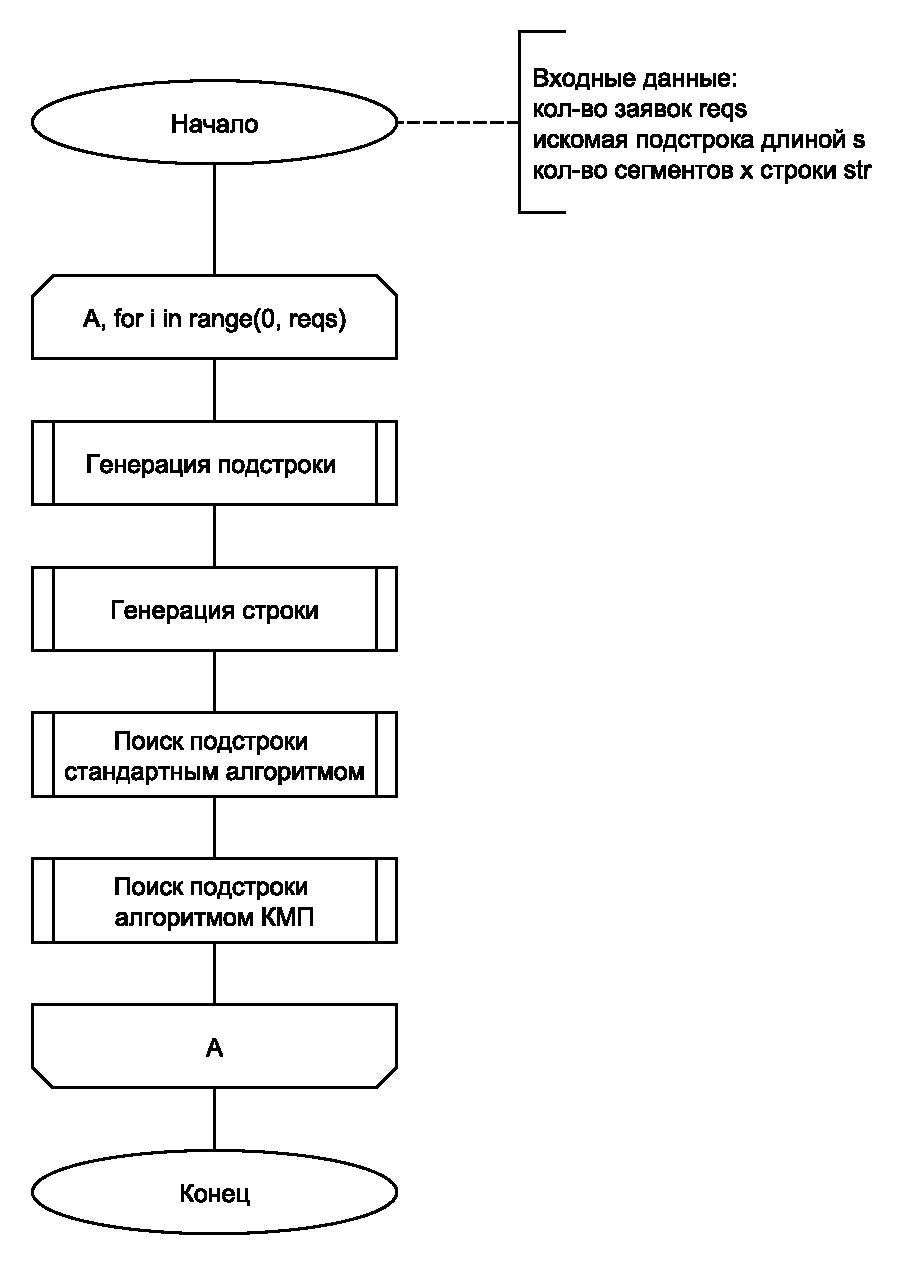
\includegraphics[width=0.7\linewidth]{images/linear}
	\caption[Последовательная обработка лент]{}
	\label{fig:linear}
\end{figure}

На рисунке \ref{fig:parallel} изображен параллельный случай реализации конвейера.
Он заключается в том, что все вторая и третья ленты выполняются одновременно в разных потоках.

\begin{figure}
	\centering
	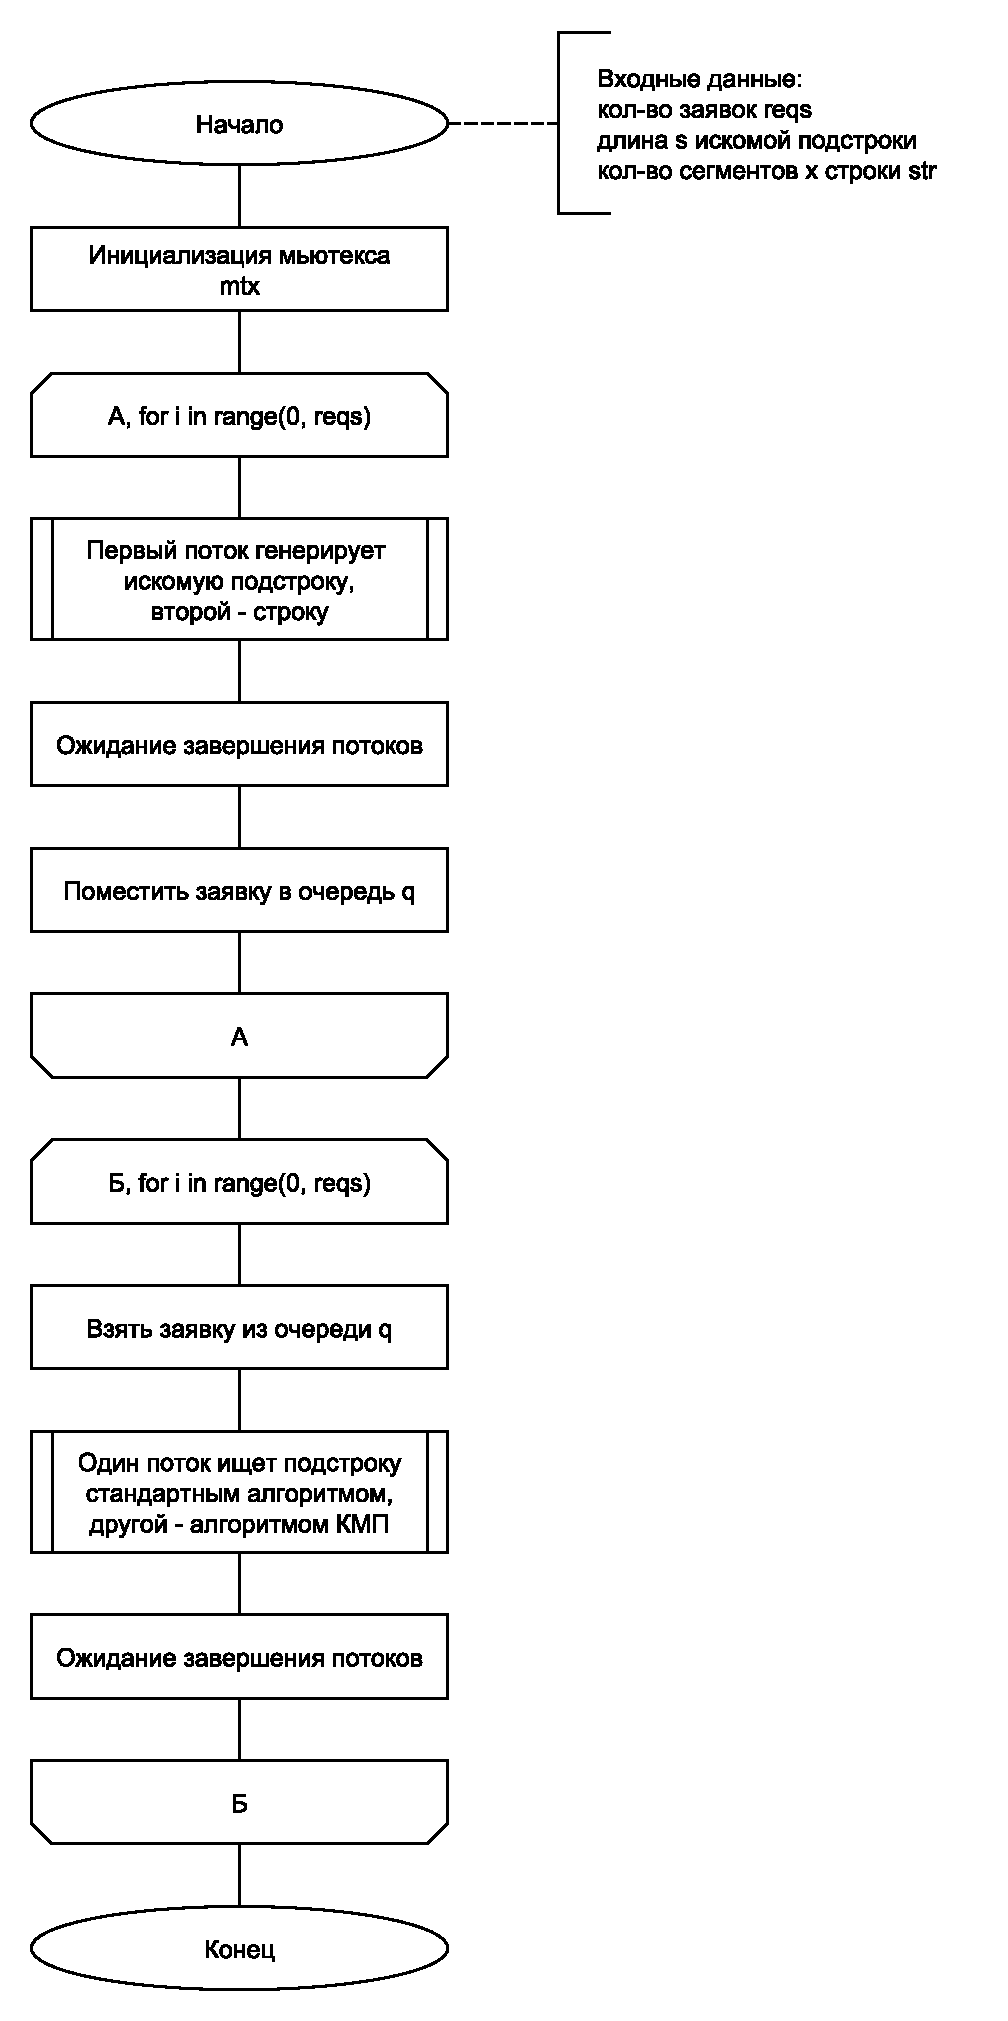
\includegraphics[width=0.7\linewidth]{images/parallel}
	\caption[Параллельная конвейерная обработка]{}
	\label{fig:parallel}
\end{figure}

При этом, функция записи лога на рисунке~\ref{fig:log} содержит критическую секцию, доступ к которой ограничивается мьютексом, который передается каждому потоку.

\begin{figure}
	\centering
	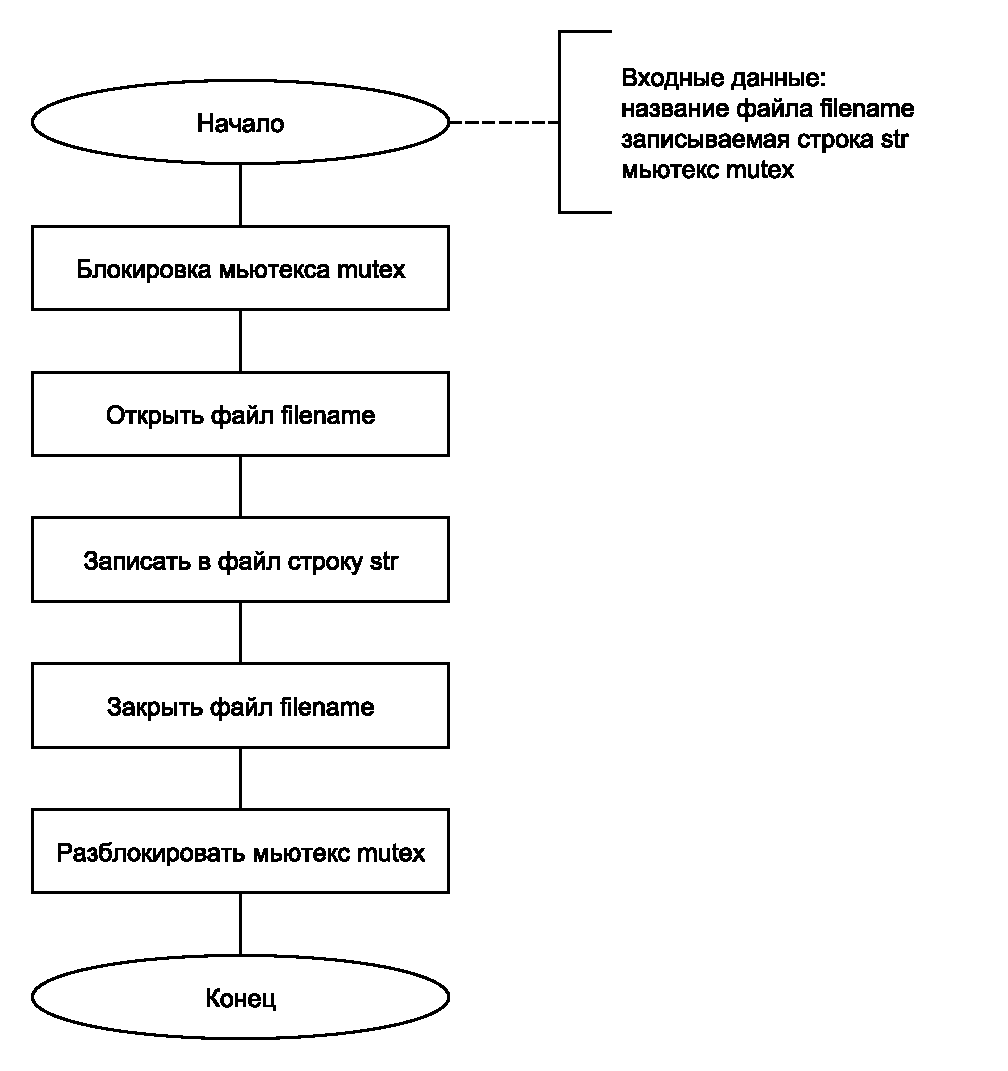
\includegraphics[width=0.7\linewidth]{images/log.pdf}
	\caption[Запись строки в файл]{}
	\label{fig:log}
\end{figure}
	\section{Технологическая часть}
В данном разделе приведены требования к программному обеспечению, средства реализации и листинги кода.

\subsection{Требования к ПО}
На вход подается строка и искомая в ней подстрока.
На выходе требуется получить индекс первого вхождения подстроки или отрицательное число, если такое не было найдено.

\subsection{Средства реализации}

В качестве языка программирования для реализации лабораторной работы был выбран Python.
Данный выбор обусловлен наличием библиотеки $time$~\cite{time} для замера времени выполнения алгоритмов.

\subsection{Сведения о модулях программы}
Программа состоит из следующих программных модулей:
\begin{enumerate}[label={\arabic*)}]
	\item standart.py --- модуль реализации стандартного алгоритма;
	\item prefix.py --- модуль реализации расчета префиксного массива;
	\item KMP.py --- модуль реализации алгоритма Кнута~--~Морриса~--~Пратта;
	\item time.py --- модуль замера времени выполнения алгоритмов;
	\item plot.py --- модуль создания графического представления значений;
	\item main.py --- модуль, содержащий меню.
\end{enumerate}

\newpage
\subsection{Реализация алгоритмов}

В листингe \ref{lst:standart} приведена реализация стандартного алгоритма поиска подстроки в строке.

\begin{lstinputlisting}[
	label={lst:standart},
	caption={Стандартный алгоритм},
	]{../src/lab_07/standart.py}
\end{lstinputlisting}

В листингe \ref{lst:prefix} приведена реализация расчета префиксного массива.

\begin{lstinputlisting}[
	label={lst:prefix},
	caption={Получение префиксного массива},
	]{../src/lab_07/prefix.py}
\end{lstinputlisting}

\newpage
В листингe \ref{lst:kmp} приведена реализация алгоритма Кнута~--~Морриса~--~Пратта.
\begin{lstinputlisting}[
	label={lst:kmp},
	firstline=4,
	caption={Алгоритм Кнута~--~Морриса~--~Пратта},
	]{../src/lab_07/kmp.py}
\end{lstinputlisting}

Алгоритм также возвращает второе значение кол-ва сравнений потому что это требуется для определения худшего случая положения искомой подстроки в тексте в исследователькой части.
	\section{Исследовательская часть}

\subsection{Технические характеристики}

Технические характеристики устройства, на котором выполнялся замерный эксперимент:
\begin{itemize}[label*=---]
	\item операционная система Windows 11;
	\item память 16 ГБ;
	\item процессор 3,6 ГГц 6-ядерный процессор AMD Ryzen 5000 series 5.
\end{itemize}

Замеры проводилось на ноутбуке, включенном в сеть электропитания. Во время тестирования ноутбук был нагружен только окружением и непосредственно выполняемой программой.

\subsection{Пример работы программы}

На рисунке \ref{img:example} представлен пример работы программы. Вводится две строки, после чего выводится результат и время работы каждого алгоритма в микросекундах. 

\begin{figure}[!h]
	\centering
	\includegraphics[width=130mm]{images/example}
	\caption{Пример работы программы}
	\label{img:example}
\end{figure}

\pagebreak
\newpage
\subsection{Время выполнения реализованных алгоритмов}

Введём следующие обозначения:
\begin{description}
	\item[Л] - Левенштейна
	\item[ДЛ] - Дамерау-Левенштейн
	\item[РДЛ] - Рекурсивный Дамерау-Левенштейн
	\item[РДЛК] - Рекурсивный Дамерау-Левенштейн с кэшем
\end{description}

\begin{table}[hbtp]
	\centering
	\caption{Результаты замеров времени реализованных алгоритмов в тактах процессора}
	\label{tab:time}
	\begin{tabular}{|r|r|r|r|r|}
		\hline
		Длина строк & Л & ДЛ & РДЛ & РДЛК \\
		\hline
		1 & $1.720 \times 10^3$ & $2.014 \times 10^3$ & $87.255 \times 10^0$ & $114.828 \times 10^0$ \\
		2 & $1.483 \times 10^3$ & $1.759 \times 10^3$ & $23.594 \times 10^0$ & $26.462 \times 10^0$ \\
		3 & $2.797 \times 10^3$ & $2.803 \times 10^3$ & $146.202 \times 10^0$ & $62.051 \times 10^0$ \\
		4 & $3.084 \times 10^3$ & $2.897 \times 10^3$ & $719.301 \times 10^0$ & $103.013 \times 10^0$ \\
		5 & $4.516 \times 10^3$ & $4.042 \times 10^3$ & $3.699 \times 10^3$ & $2.098 \times 10^3$ \\
		6 & $3.984 \times 10^3$ & $3.984 \times 10^3$ & $17.288 \times 10^3$ & $20.112 \times 10^3$ \\
		7 & $3.785 \times 10^3$ & $3.513 \times 10^3$ & $83.077 \times 10^3$ & $24.901 \times 10^3$ \\
		8 & $6.053 \times 10^3$ & $5.256 \times 10^3$ & $553.444 \times 10^3$ & $6.769 \times 10^3$ \\
		9 & $8.088 \times 10^3$ & $5.973 \times 10^3$ & $2.640 \times 10^4$ & $8.404 \times 10^3$ \\
		10 & $8.570 \times 10^3$ & $6.942 \times 10^3$ & $1.433 \times 10^5$ & $11.075 \times 10^4$ \\
		\hline
	\end{tabular}
\end{table}

Замеры времени работы реализованных алгоритмов для определенной длины строк проводились 100 раз, при этом каждый раз строки генерировались случайно. В качестве результата, представленного в таблице \ref{tab:time}, взято среднее время на каждой длине слова.

\pagebreak
\newpage

\subsection{Занимаемая память реализованных алгоритмов}

В данном разделе представлены результаты замеров затрат памяти для различных алгоритмов на обработку строк разной длины. Таблица \ref{tab:memory} демонстрирует объем памяти в байтах, потребляемый разными реализациями алгоритмов в зависимости от длины обрабатываемых строк.

\begin{table}[ht]
	\label{tab:memory}
	\begin{center}
		\caption{Затраты памяти в байтах для различных алгоритмов в зависимости от длины строк }
		\begin{tabular}{|c|c|c|c|c|}
			\hline
			N & Л & ДЛ & РДЛ & РДЛК \\
			\hline
			1  & 28  & 28  & 32  & 64  \\
			2  & 48  & 48  & 32  & 140  \\
			3  & 76  & 76  & 32  & 224  \\
			4  & 112 & 112 & 32  & 352  \\
			5  & 156 & 156 & 32  & 544  \\
			6  & 208 & 208 & 32  & 800  \\
			7  & 268 & 268 & 32  & 1088  \\
			8  & 336 & 336 & 32  & 1376  \\
			9  & 412 & 412 & 32  & 1696  \\
			10 & 496 & 496 & 32  & 2032  \\
			\hline
		\end{tabular}
		\label{tab:memory}
	\end{center}
\end{table}

\subsection{Сравнительный анализ алгоритмов}

	Рекурсивная реализация алгоритма Дамерау-Левенштейна (РДЛ) демонстрирует значительно худшую производительность по времени выполнения по сравнению с итеративными алгоритмами. Рекурсивные алгоритмы следует использовать только для обработки строк крайне малой длины (1-2 символа) или в ситуациях, когда доступно ограниченное количество оперативной памяти.
	
	Алгоритм Дамерау-Левенштейна (ДЛ) и итеративная реализация с кэшированием (РДЛК) подходят для обработки строк разной длины. Однако следует обратить внимание, что ДЛ затрачивает больше памяти по сравнению с РДЛК, особенно при работе с длинными строками. РДЛК является предпочтительным выбором, когда требуется учитывать ошибки, связанные с транспозицией символов, и при этом ограничены объемы доступной памяти.
	Несмотря на увеличение затрат памяти при использовании итеративных алгоритмов, они предоставляют хорошую скорость выполнения, особенно при обработке строк средних и больших размеров.
	
	В случаях, когда расстояние Дамерау-Левенштейна играет важную роль из-за ошибок, связанных с транспозицией символов, алгоритм Дамерау-Левенштейна (ДЛ и РДЛК) является наиболее предпочтительным выбором, несмотря на некоторое увеличение временных и памятных затрат.

\subsection{Вывод}

В результате анализа замеров времени выполнения и затрат памяти на различных алгоритмах были сделаны следующие выводы:

\begin{itemize}
	\item Для обработки строк малой длины и при ограниченных объемах памяти рекомендуется использовать рекурсивные алгоритмы.
	\item Для строк средних и больших размеров и при наличии достаточной памяти, итеративные алгоритмы предоставляют лучшую производительность.
	\item При необходимости учета транспозиций символов и ограниченных ресурсах памяти алгоритм Дамерау-Левенштейна с кэшированием (РДЛК) является предпочтительным выбором.
\end{itemize}

В конечном итоге, выбор подходящего алгоритма зависит от требований вашей задачи, доступных ресурсов памяти и желаемой скорости выполнения.

	\section*{ЗАКЛЮЧЕНИЕ}
\addcontentsline{toc}{section}{ЗАКЛЮЧЕНИЕ}

Цель работы достигнута: описаны последовательные и параллельные конвейерные вычисления нахождения подстроки в строке стандартным алгоритмом и алгоритмом Кнута~---~Морриса~---~Пратта (КМП), проведено сравнение времени работы.

В ходе выполнения лабораторной работы были решены все задачи:
\begin{itemize}
	\item описана структура конвейерной обработки данных;
	\item описаны и реализованы используемые алгоритмы;
	\item определены средства программной реализации;
	\item реализована программа, выполняющая заданную конвейерную обработку;
	\item проведено сравнение реализаций алгоритмов по затраченному времени;
	\item подготовлен отчет по лабораторной работе.
\end{itemize}

В результате исследования выяснилось, что для задачи поиска подстроки в строке с помощью конвейерной обработки следует использовать последовательную реализацию, поскольку она быстрее параллельной при кол-ве заявок до 1000. 
В среднем выигрышь составляет 40\%.

	\printbibliography
	
	
\end{document}